\chapter{Meilenstein II}
\label{cha:ms2}

Der zweite Meilenstein dient zur Einführung in Werkzeuge und Funktionalitäten des Semantic Web. Obwohl gruppenspezifische Projekte entwickelt werden sollen, sind alle Gruppen in der Lage ihre Aktoren und Sensoren als Ressourcen im Netzwerk zur Verfügung zu stellen. Eine gegebene Ontologie, siehe Bild \ref{img:ontology}, wird gruppenübergreifend erweitert um einheitlichen Zugriff zu gewährleisten.


\begin{figure}
	\centering
	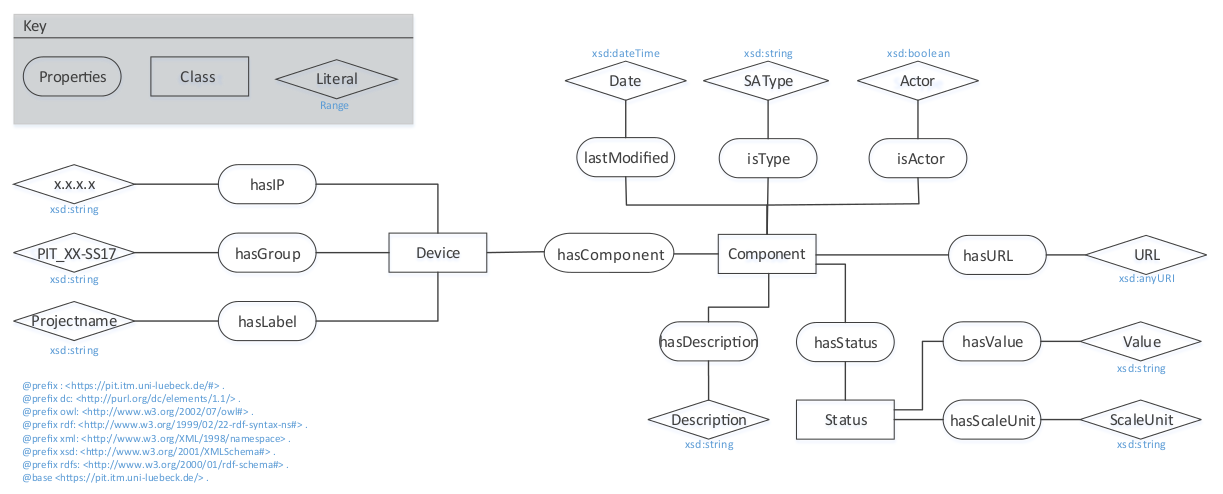
\includegraphics[width=1\textwidth]{figures/ontology.png}
	\caption{Turtle Ontology zur Verwendung und Erweiterung im Rahmen des Projekts}
	\addloflink{https://moodle.uni-luebeck.de/pluginfile.php/112836/mod_resource/content/7/handbuch.pdf}
	\label{img:ontology}
\end{figure}



\section{COAP2SSP}
\label{sec:coap2ssp}

Um sich mit der Ansteuerung des SSP vertraut zu machen, soll in der ersten Teilaufgabe des zweiten Meilensteins ein einfacher observierbarer Zeitservice implementiert werden. Als Vorlage dient die Beispielanwendung im bereitgestellten nCoAP Paket, wie beschrieben in Abschnitt \ref{subsec:ncoap}. Die Klasse \textit{SimpleObservableTimeService} erweitert dazu den vorgegebenen \textit{SimpleObservableService} und besteht aus drei wesentlichen Abschnitten. Das Datenformat des Services wird durch Ontologien vorgegeben und in Listing \ref{code:sots_ontology} initialisiert. Von besonderem Interesse ist hier der Punkt \textit{ContentFormat.APP\_TURTLE} da es sich dabei um die im Projekt zu verwendende Beschreibungsform handelt.


\begin{lstlisting}[float=htb,caption={SimpleObservableTimeService Beschreibung der Payload},label=code:sots_ontology]
static{
        payloadTemplates.put(
                ContentFormat.TEXT_PLAIN_UTF8,
                "The current time is %02d:%02d:%02d"
        );
        
        payloadTemplates.put(
	        ContentFormat.APP_TURTLE,
	        "@prefix itm: <http://gruppe04.pit.itm.uni-luebeck.de/>\n" +
	        "@prefix xsd: <http://www.w3.org/2001/XMLSchema#>\n" +
	        "\n" + 
	        "itm:time1 itm:hour \"%02d\"^^xsd:integer .\n" + 
	       	"itm:time1 itm:minute \"%02d\"^^xsd:integer .\n" + 
	       	"itm:time1 itm:seconds \"%02d\"^^xsd:integer ."
        );        
    }
\end{lstlisting}

% **********

Der Konstruktor der Klasse, im Listing \ref{code:sots_constructor}, erhält als Übergabeparameter zum Einen den eindeutigen Bezeichner der neuen Ressource und zum Anderen das vorgesehene Aktualisierungsintervall. 

\begin{lstlisting}[float=htb,caption={Konstruktor mit Ressourcenpfad und Updateintervall},label=code:sots_constructor]
/**
     * Creates a new instance of {@link SimpleObservableTimeService}.
     *
     * @param path the path of this {@link SimpleObservableTimeService} (e.g. /utc-time)
     * @param updateInterval the interval (in seconds) for resource status updates (e.g. 5 for every 5 seconds).
     */
    public SimpleObservableTimeService(String path, int updateInterval, ScheduledExecutorService executor) {
        super(path, updateInterval, executor);
    }
\end{lstlisting}

% **********

Mit der Funktion \textit{getSerializedResourceStatus(long contentFormat)} in Listing \ref{code:sots_update} wird die Updatefunktion der Ressource definiert. Als Rückgabewert wird ein String der gewählten Nachrichtenform mit den aktualisierten Informationen ausgegeben.

\begin{lstlisting}[float=htb,caption={Updatefunktiondes Services},label=code:sots_update]
    @Override
    public byte[] getSerializedResourceStatus(long contentFormat) {
        LOG.debug("Try to create payload (content format: " + contentFormat + ")");

        String template = payloadTemplates.get(contentFormat);
        if (template == null) {
            return null;
        } else {
            long time = getResourceStatus() % 86400000;
            long hours = time / 3600000;
            long remainder = time % 3600000;
            long minutes = remainder / 60000;
            long seconds = (remainder % 60000) / 1000;
            return String.format(template, hours, minutes, seconds).getBytes(CoapMessage.CHARSET);
        }
    }
\end{lstlisting}

Nachdem die Ressource definiert wurde, braucht es zum Abschluss der ersten Teilaufgabe noch einen CoAP-Endpoint. Dieser Dienst wird auf dem Raspberry Pi ausgeführt und meldet sich am SSP an um dort seine definierten Ressourcen zu registrieren. Zu diesem Zweck müssen Adresse und Port des SSP beschrieben werden, wie in Listing \ref{code:sots_ssp_interface} dargestellt. Weiterhin benötigt der Endpoint Instanzen der ihm zugeordneten Ressourcen, d.h. Methoden um die entsprechenden Konstruktoren auszuführen. Schließlich erfolgt die Anmeldung am SSP mittels {registerAtSSP()}, welches in Listing \ref{code:sots_ssp_registry} wiedergegeben wird.


\begin{lstlisting}[float=htb,caption={Definition der SSP Schnittstelle},label=code:sots_ssp_interface]

@Option(name = "--host", usage = "Host of the SSP (ip or domain)")
	private String SSP_HOST = "141.83.151.196";

@Option(name = "--port", usage = "Port of the SSP")
	private int SSP_PORT = 5683;

\end{lstlisting}


% **********


\begin{lstlisting}[float=htb,caption={Registrierung am SSP},label=code:sots_ssp_registry]
public void registerAtSSP() throws URISyntaxException {
        URI resourceURI = new URI ("coap", null, SSP_HOST, SSP_PORT, "/registry", null, null);
        CoapRequest coapRequest = new CoapRequest(MessageType.CON, MessageCode.POST, resourceURI);
        InetSocketAddress remoteSocket = new InetSocketAddress(SSP_HOST, SSP_PORT);

        SimpleCallback callback = new SimpleCallback();
        this.sendCoapRequest(coapRequest, remoteSocket, callback);
}
\end{lstlisting}

Zum Abschluss der Aufgabe kann, mit Hilfe des Browser-Plugins Copper, direkt am Endpoint getestet werden, ob alle Funktionen ausgeführt werden. Mit dem gegebenen SPARQL-Endpoint \url{http://141.83.151.196:8080/services/ sparql-endpoint} wird sichergestellt, dass die Ressourcen auch am SSP korrekt registriert werden. Dies ist auch der erste Punkt um sich aktiv mit einer SPARQL-Query auseinander zu setzen und so die Vorbereitung für die zweite Teilaufgabe einzuleiten.

\section{SSP2PI}
\label{sec:ssp2pi}

In der zweiten Teilaufgabe des Meilensteins wird die entwickelte Anwendung um die berechneten Lux-Werte des ersten Meilensteins erweitert. Dazu wird eine weitere beobachtbare Ressource, basierend auf vorgegebener Ontologie \ref{img:ontology}, zu dem Programm hinzugefügt. In Codebeispiel \ref{code:sols_ontology} ist die Beschreibung der Payload dargestellt. Wieder ist das Turtle-Format von besonderem Interesse, da hier sehr gut nachvollziehbar ist wie die gegebene Ontology praktisch umgesetzt wird. Bei der Implementierung wurden zwei Hürden indentifiziert. Zum Einen muss bei der Definition der Präfixe präzise darauf geachtet werden die korrekte URI zu verwenden. Wird Beispielsweise das Präfix \textit{pit} mit \url{http://pit.itm...} statt mit \url{https://pit.itm...} beschrieben so handelt es sich für die Anwendung um eine andere Quelle und die Ressource wird, trotz korrekter Anfrage, nicht gefunden werden. Zum Anderen müssen Daten entsprechend ihrer Beschreibung formatiert werden. Das Attribut \textit{pit:lastModified} ist vom Typ \textit{xsd:dateTime}, welches die Form \textit{YYYY-MM-TT'T'HH:mm:ss} hat. Bei Abweichung von dem Format wird sich die Ressource nicht am SSP registrieren lassen. Die weitere Implementierung dieser Ressource folgt unumwunden dem Ablauf der ersten Teilaufgabe.

\begin{lstlisting}[float=htb,caption={SimpleObservableLuxService Beschreibung der Payload},label=code:sols_ontology]
static{
        payloadTemplates.put(
                ContentFormat.TEXT_PLAIN_UTF8,
                "The current ldr is %a"
        );

        payloadTemplates.put(
	        ContentFormat.APP_TURTLE,
	        "@prefix itm: <http://gruppe04.pit.itm.uni-luebeck.de/>\n" +
	        "@prefix pit: <https://pit.itm.uni-luebeck.de/>\n" +
	        "@prefix xsd: <http://www.w3.org/2001/XMLSchema#>\n" +
			"\n" + 
	        "itm:ldr pit:hasDescription \"Sensor for Lux value\"^^xsd:string ." +
	        "\n" + 
			"itm:ldr pit:hasURL \"http://gruppe04.pit.itm.uni-luebeck.de/ldr\"^^xsd:anyURI ." +
			"\n" + 
			"itm:ldr pit:isActor \"false\"^^xsd:boolean ." +
			"\n" + 
			"itm:ldr pit:isType \"LDR\"^^xsd:string ." +
			"\n" + 
	        "itm:ldr pit:hasStatus itm:ldrStatus ." +
			"\n" + 
	        "itm:ldr pit:lastModified \"%s\"^^xsd:dateTime ." +			
	        "\n" + 
	        "itm:ldrStatus pit:hasScaleUnit \"Lux\"^^xsd:string ." +
	        "\n" +
	        "itm:ldrStatus pit:hasValue \"%s\"^^xsd:string ."
        );        
    }
\end{lstlisting}

Schließlich soll mittel SPARQL-Querry eine Abfrage an den SSP gesendet werden um den Durchschnitt aller registrierten Lux-Werte abzufragen und eine LED entsprechend anzusteuern. Zu diesem Zweck wird ein HTTP-Client benötigt, der die in \ref{code:sols_sparql} Abfrage an den SSP sendet und die Antwort entsprechend auswertet.

\begin{lstlisting}[float=htb,caption={SPARQL-Query zur Ermittlung des durchschnittlichen Lux-Wertes},label=code:sols_sparql]
String sparql = "PREFIX itm: <http://gruppe04.pit.itm.uni-luebeck.de/> \n" +
				"PREFIX  pit: <https://pit.itm.uni-luebeck.de/>\n" +
				"PREFIX  xsd: <http://www.w3.org/2001/XMLSchema#>\n" +
				"\n" + 
				"Select (AVG(xsd:float(?v)) as ?luxAverage)  \n" + 
				"Where{ \n" +
				"?o pit:isType \"LDR\"^^xsd:string . \n" +
				"?o pit:hasStatus ?p . \n" +
				"?p pit:hasValue ?v . \n" +
				"}";
\end{lstlisting}




%The following is just a further quick link list compiled to help in creating good scientific presentations.
%\begin{itemize}
%\item \url{http://www.the-scientist.com/?articles.view/articleNo/28818/title/Pimp-your-PowerPoint/}
%\item \url{http://www.northwestern.edu/climb/resources/oral-communication-skills/creating-a-presentation.html}
%\item \url{http://www.nextscientist.com/improve-presentation-skills-of-phd-students/}
%\end{itemize}


%%%%% Emacs-related stuff
%%% Local Variables: 
%%% mode: latex
%%% TeX-master: "../../main"
%%% End: 
